% Name: Sun
% Description: Five kites meeting at their 72° tips, one of the seven ways Penrose tiles can surround a vertex, with the matching arcs joining into circles.
% Tags: penrose, kite, vertex configuration, sun

\usetikzlibrary{tilings.penrose}

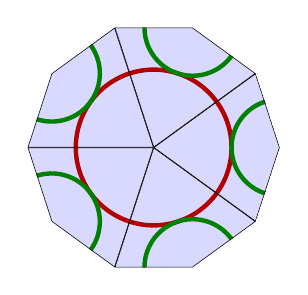
\begin{tikzpicture}[
  every tile pic/.style={transform shape},
  every tile/.style={draw},
  every circle arc/.style={draw=red!70!black, ultra thick},
  every long arc/.style={draw=green!50!black, ultra thick},
  scale=1.6,
]
  % fill the five kites first, then draw them again with their arcs on top
  \foreach \k in {0,...,4} {
    \pic[kite, rotate=72*\k, every tile/.style={fill=blue!15}];
  }
  \foreach \k in {0,...,4} {
    \pic[kite, rotate=72*\k];
  }
\end{tikzpicture}
